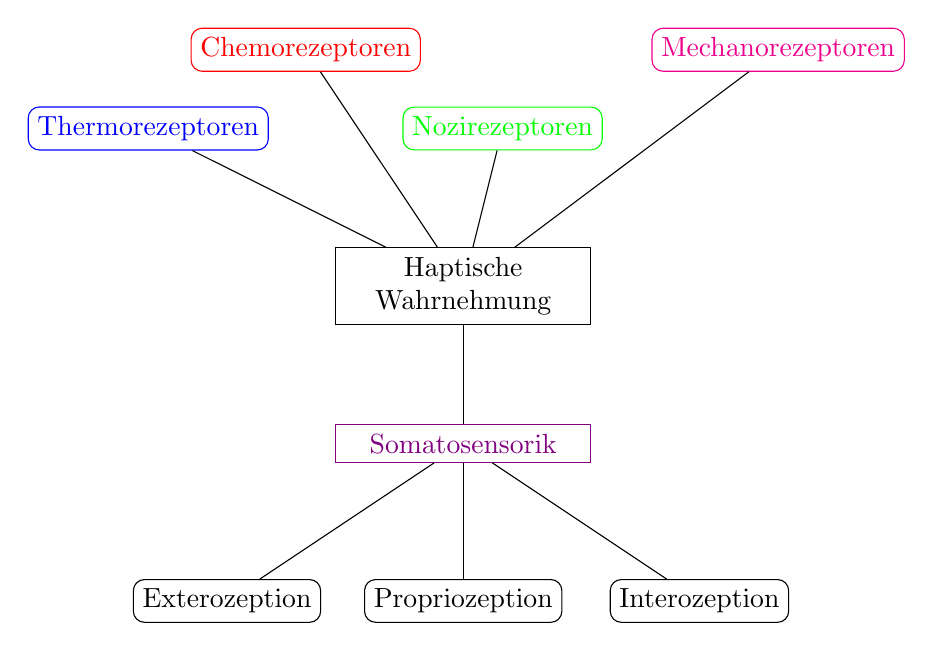
\begin{tikzpicture}[first style/.style={rectangle, draw, rounded corners, align=center}, steuer style/.style={draw, rectangle, text width=3cm, align=center}]
	\node[steuer style] (S1) at (0, 0) {Haptische Wahrnehmung};
	\node[steuer style, violet] (S2) at (0, -2) {Somatosensorik};
	\node[first style] (S3) at (-3, -4) {Exterozeption};
	\node[first style] (S4) at (0, -4) {Propriozeption};
	\node[first style] (S5) at (3, -4) {Interozeption};
	\node[first style, blue] (S6) at (-4, 2) {Thermorezeptoren};
	\node[first style, red] (S7) at (-2, 3) {Chemorezeptoren};
	\node[first style, green] (S8) at (0.5, 2) {Nozirezeptoren};
	\node[first style, magenta] (S9) at (4, 3) {Mechanorezeptoren};
	\draw (S1) -- (S2);
	\foreach \y in {3,...,5}
	\draw (S2) -- (S\y);
	\foreach \x in {6,...,9}
	\draw (S1) -- (S\x);
\end{tikzpicture}